\documentclass[11pt]{article}
\usepackage[shortlabels]{enumitem}
\usepackage[margin=1in,headheight=15pt]{geometry}   % Adjusted headheight
\usepackage{amsmath}
\usepackage{fancyhdr}
\usepackage{graphicx}
\usepackage{cancel}
\usepackage{amsfonts}
\usepackage{setspace}

% Set up fancy header/footer
\pagestyle{fancy}
\fancyhead[LO,L]{Jimmy Chen}
\fancyhead[CO,C]{CSCI 2500 - Computer Organization}
\fancyhead[RO,R]{November 30, 2023}
\fancyfoot[LO,L]{}
\fancyfoot[CO,C]{\thepage}
\fancyfoot[RO,R]{}
\renewcommand{\headrulewidth}{0.4pt}
\renewcommand{\footrulewidth}{0.4pt}
\graphicspath{ {./images/} }
\onehalfspacing

\begin{document}
\section{Homework 4}


\setcounter{section}{12}
\setcounter{subsection}{13}
\subsection{Excersises}

\setcounter{subsubsection}{4}
\subsubsection{Question 5}
In the exercise, we examine in detail how an instruction is executed in single-cycle datapath. Problems in this exercise refer to a clock cycle in which the processor fetches the following instruction word: 0xadac0014.\\
For context: The encoded instruction is \textbf{sw \$t4, 20(\$t5)}

\begin{enumerate}[(a)]
    \item What are the values of the ALU control unit's inputs for this instruction?\\
    \textbf{Work:}
    \begin{center}
        Opcode: 0xadac // Opcode for sw\\
        Source Register (\$t5)\\
        Destination Register (\$t4)\\
        Offset: 20\\
        ALUOperation: 10 (Add)\\
        ALUSrc (ALU source): 1 (Immediate value from instruction)\\
        Function: 0 (Not used)\\
        \fbox{\begin{minipage}{24em}
            \begin{center}
                \Large{\textbf{Answer: ALU Control Input: 101}}
            \end{center}
        \end{minipage}}
    \end{center}

    \item What is the new PC address after this instruction is executed? Highlight the path through which this value is determined.\\
    \textbf{Work:}
    \begin{center}
        ALU operand 1: PC value\\
        ALU operand 2: 4 // Constant value to add \\
        \fbox{\begin{minipage}{35em}
            \begin{center}
                \Large{\textbf{Answer: The new will be the old PC address + 4.}}
            \end{center}
        \end{minipage}}
    \end{center}

    \item For each mux, show the values of its inputs and outputs during the execution of this instruction. List values that are register outputs at \textbf{Reg [xn]}\\
    \textbf{Work:}\\[0.15in]
    Mux1 (ALU Source):
    \begin{itemize}
        \item Input 0: PC + 4
        \item Input 1: Sign-extended offset
        \item Output: Sign-extended offset
    \end{itemize}
    Mux2 (Write Register):
    \begin{itemize}
        \item Input 0: Register \$t4's number // dest reg
        \item Input 1: Register \$t5's number // src reg
        \item Selected Input: 0 // since we're writing to \$t4
    \end{itemize}
    Mux3 (Write Data):
    \begin{itemize}
        \item Input 0: ALU result // memory address to store data
        \item Input 1: Register \$t4's value // data to be stored in memory
        \item Selected Input: 1 // since we're writing to \$t4
    \end{itemize}

    \item What are the input values for the ALU and the two add units?\\
    \textbf{Work:}
    \item What are the values of all inputs for the registers unit?\\
    \textbf{Work:}
\end{enumerate}


\setcounter{subsubsection}{6}
\subsubsection{Question 7}
Problems in this exercise assume that the logic blocks used to implement a processor's datapath (COD Figure 4.21) have the following latencies:
\begin{center}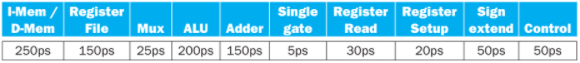
\includegraphics[scale=0.6]{q7_image}\\\end{center}
"Register read" is the time needed after the rising clock edge for the new register value to appear on the output. This value applies to the PC only. "Register setup" is the amount of time a register's data input must be stable before the rising edge of the clock. This value applies to both the PC and Register File.

\begin{enumerate}[(a)]
    \item What is the latency of an R-type instruction(i.e., how long must the clock period be to ensure that this instruction works correctly)?
    \item What is the latency of lw? (Check your answer carefully. Many students place extra muxes on the critical path.)
    \item What is the latency of sw? (Check your answer carefully. Many students place extra muxes on the critical path.)
    \item What is the latency of beq?
    \item What is the latency of an arithmetic, logical, or shift I-type (non-load) instruction?
    \item What is the minimum clock period for this CPU?
\end{enumerate}


\setcounter{subsubsection}{9}
\subsubsection{Question 10}
When the processor designers consider a possible improvement to the processor datapath, the decision usually depends on the cost/performance trade-off. In the following three problems, assume that we are beginning with the datapath from COD figure 4.21, the latencies from Exercise 4.7, and the following costs:
\begin{center}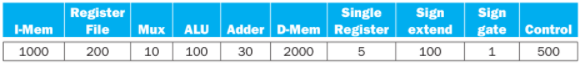
\includegraphics[scale=0.6]{q10_image}\\\end{center}
Suppose doubling the number of general purpose registers from 32 to 64 would reduce the number of lw and sw instruction by 12\%, but increase the latency of the register file from 150 ps to 160 ps and double the cost from 200 to 400. (Use the instruction mix from Exercise 4.8 and ignore the other effects on the ISA discussed in Exercise 2.18.)

\begin{enumerate}[(a)]
    \item What is the speedup achieved by adding this improvement?
    \item Compare the change in performance to the change in cost.
    \item Given the cost/performance ratios you just calculated, describe a situation where it makes sense to add more registers and describe a situation where it doesn't make sense to add more registers.
\end{enumerate}


\setcounter{subsubsection}{15}
\subsubsection{Question 16}
In this exercise, we examine how pipelining affects the clock cycle time of the processor. Problems in this exercise assume that individual stages of the datapath have the following latencies:
\begin{center}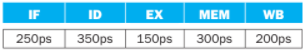
\includegraphics[scale=0.68]{q16_image1}\\\end{center}
Also, assume that instructions executed by the processor are broken down as follows:
\begin{center}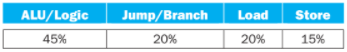
\includegraphics[scale=0.6]{q16_image2}\\\end{center}

\begin{enumerate}[(a)]
    \item What is the clock cycle time in a pipelined and non-pipelined processor?
    \item What is the total latency of an lw instruction in a pipelined and non-pipelined processor?
    \item If we can split one stage of the pipelined datapath into two new stages, each with half the latency of the original stage, which stage would you split and what is the new clock cycle time of the processor?
    \item Assuming there are no stalls or hazards, what is the utilization of the data memory?
    \item Assuming there are no stalls or hazards, what is the utilization of the write-register port of the "Registers" unit?

\end{enumerate}
\end{document}